%%%
% Tech report template. Compile with pdflatex
%%%
%\documentclass[pdftext,twoside,12pt]{report}
\documentclass[pdftext,twoside,11pt]{article}

\usepackage[a4paper,lmargin=2.5cm,rmargin=2cm,tmargin=1cm,bmargin=1cm,includehead,includefoot]{geometry}
\usepackage[german,english]{babel}
\usepackage{url}
\usepackage{subfig}
\usepackage{fancyhdr}
\usepackage{caption}
\usepackage{array}
\usepackage{amsmath} % needed for subequations
\usepackage{amssymb}
\usepackage{marvosym} % for the Euro symbol
\usepackage{mathptmx}
\usepackage{multirow}
\usepackage[small,compact]{titlesec}  %for compressed Section titles
\usepackage{mdwlist}  %for compressed itemized lists
\usepackage{setspace} %for chaging spacing in environments (see biblio)
\usepackage[numbers,sort&compress]{natbib}
\usepackage[scaled=.90]{helvet}
\usepackage{times}
\usepackage[T1]{fontenc}
%\usepackage[latin1]{inputenc}
\usepackage[utf8]{inputenc}
\usepackage{graphicx} 
\usepackage{pgf}
\usepackage{hypernat}
\usepackage{hyperref}

%%% Package options %%%

\hypersetup{colorlinks=true, breaklinks=true, pagebackref=true,
  urlcolor=blue, linkcolor=blue,anchorcolor=blue,citecolor=blue,
  pdfpagemode = UseNone, %FullScreen, %UseThumbs, %UseOutlines,
  pdfauthor = {},
  pdftitle = {},   
  pdfsubject = {},
  pdfkeywords = {}
}

\DeclareGraphicsExtensions{.jpg,.pdf,.mps,.png}
\graphicspath{{img/} {./}} %put all figures in these dirs

\urlstyle{rm} %so it doesn't use a typewriter font for urls.

%\newcommand{\bibfont}{\scriptsize} %for smaller fonts in biblio

\renewcommand{\captionfont}{\small \sffamily}

\renewcommand\floatpagefraction{.9}
\renewcommand\topfraction{.9}
\renewcommand\bottomfraction{.9}
\renewcommand\textfraction{.1}   

\setlength{\bibsep}{1pt}           %for compressed itemized list on biblio
\setlength{\topsep}{0pt}
\setlength{\itemsep}{0pt}
\setlength{\partopsep}{0pt}
\setcounter{totalnumber}{50}
\setcounter{topnumber}{50}
\setcounter{bottomnumber}{50}

%Example of image declaration (declared once in pdf file, reduces file size)
%\pgfdeclareimage[height=0.8cm]{logo}{img/logo} 
%Use with:
%\pgfuseimage{logo}

% Headers and Footers
\pagestyle{fancy}
\fancyhead{} % reset headers
\fancyfoot{} % reset footers
\fancyhead[LO]{\textsf{\textbf{TITLE}}}
\fancyhead[CO]{\date{\today}}
\fancyhead[RO]{AUTHOR}
% remove horizontal lines between text and headers and footers
\renewcommand{\footrulewidth}{0pt}
\renewcommand{\headrulewidth}{0pt}


%  Title page
\title{A Review of Recent Research in Extracting Information From Medical Textual Documents}
\author{AUTHOR\\
  University of Florida\\
}
\date{\today}


\begin{document}

%\thispagestyle{empty}
\maketitle

% keywords

% Use with {report} documentclass
% \chapter{The beginning}
% \label{cha:beginning}

%----------------------------------------------------------%
\section{Automated identification of extreme-risk events in clinical incident reports}
\label{sec:intro} 
\begin{itemize}
\item Objectives: classification problem
\item Methods: Naive Bayes and Support Vector Machine. 
\item Result assessments: precision,recall,F-measure,AUC.
\item Feature extraction:  Punctuation removed, converted to lower case,'bags of words'
\item Input representation: binary,term-frequency, thresholding,tf-idf
\item Feature selection: excluding words in similar frequency(dimensionality reduction)
                              excluding determiners, prepositions, pronouns, conjunctions(pos tagging)
                              stemming, bigrams.
\item Training and validating the classifiers: Naive Bayes, SVM(linear,Polynomial,RBF), 10-fold cross-validation.
\end{itemize}
\section{Extracting Information from Textual Documents
 in the Electronic Health Record:A Review of Recent Research.}
\label{sec:intro} 
\begin{itemize}
\item Spell checking, word sense disambiguation(?), POS, Contextual features like negation, temporarily, and subject identification.

\item Automatic de-identification uses the extraction of personal information before its removal. Rule-based NER.
\item Contextual Feature Detection and Analysis.
             Negation(e.g. “denies any chest pain”) temporarily(e.g. “fracture of the tibia 2 years ago”). Event subject identification(e.g. “his mother has diabetes”). 
                          NegExpanding,NegEx,Negfinder: a program detecting negation terms 
                          TimeText detected temporal relations. 
\end{itemize}

\section{UMLS project}
\label{sec:intro} 
\begin{itemize}
\item The UMLS project is an effort to overcome two significant
 barriers to effective retrieval of machine-readable information. 
\item  The first is the variety of ways the same concepts are expressed
        in different machine-readable sources and by different people. disparate databases and systems.
\end{itemize}

\section{Automated systems to identify relevant
documents in product risk management}
\label{sec:intro} 
\begin{itemize}
\item  logistic regression, K-nearest neighbour, Naive Bayes, SVM
\item  Word occurrence, Binary frequence, TF-IDF. 
\item  stemming, remove prepositions, indentify acronums, synonyms obtained from Omniviz.
\end{itemize}
\section{De-Indentification}
\label{sec:intro} 
\begin{itemize}
\item  Patient's and doctor's first and last names 
\item  Id numbers, Phone, fax, pager numbers, Hospital names, Geographic locations, Dates, Ages above 90 
\end{itemize}
features of the text used in de-identification
\begin{itemize}
\item Target word to be classified
\item Words up to 2 words left/right of target
\item Target part of speech
\item Target capitalization
\item Target length and others.  
\end{itemize}
\section{Coreference resolution: A review of general methodologies and applications
in the clinical domain, Journal of Biomedical Informatics, 2011}
\label{sec:intro} 
\begin{itemize}
\item  extract drug names and signatures. extract principal diagnosis from discharge summary.
       smoking status and medication dosage, frequency, and route.
\item
\begin{center}
  %\begin{multicols}{2}
      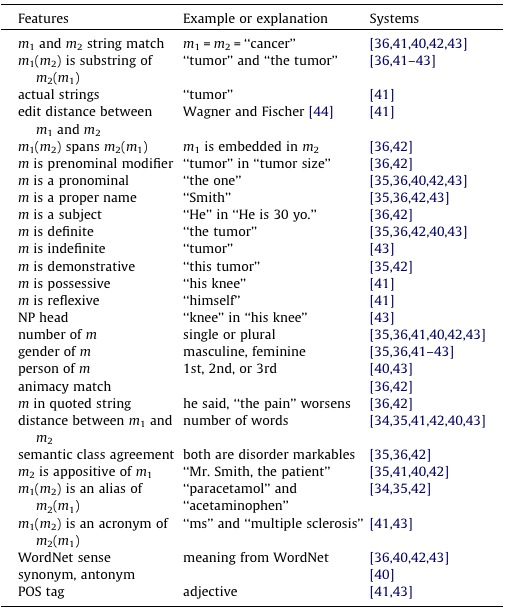
\includegraphics[height=30em,width=20em]{feature.jpg}
      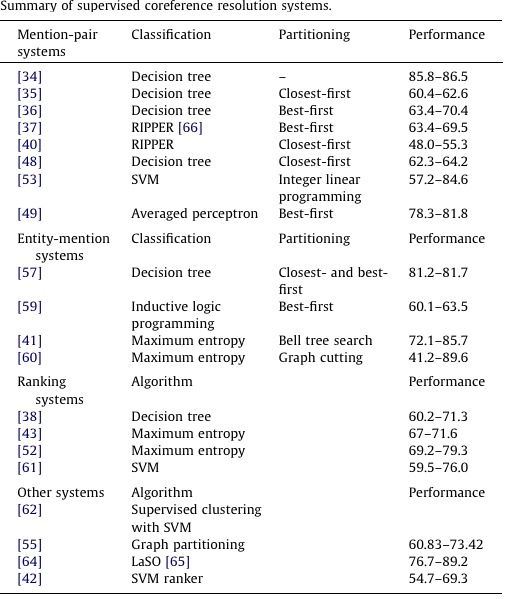
\includegraphics[height=30em,width=20em]{comparision.jpg}
  %\end{multicols}
\end{center}

\item   combined with Andrew MacCallum's most recent work, UMLS,MetaMap,and our system? 

\end{itemize}
\section{Lexical patterns, features and knowledge resources for coreference resolution
in clinical notes}
\label{sec:intro} 
\begin{center}
  %\begin{multicols}{2}
      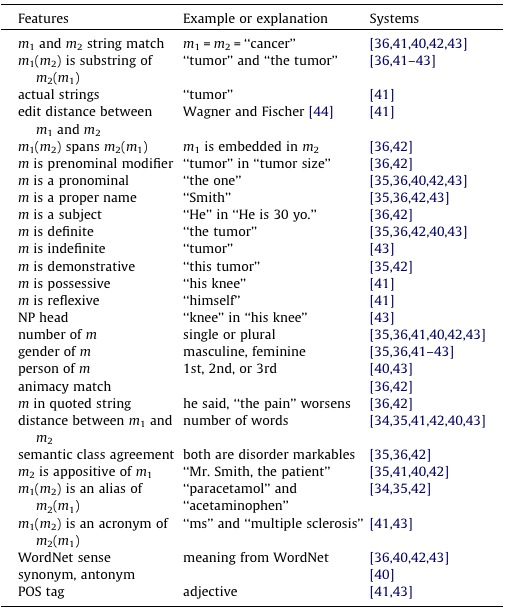
\includegraphics[height=30em,width=20em]{feature.jpg}
  %\end{multicols}
\end{center}

\item   combined with Andrew MacCallum's most recent work, UMLS,MetaMap,and our system? 
\end{itemize}
%----------------------------------------------------------%

\end{document}

